\chapter{Simulation von Streubildern}
Das Problem der Berechnung synthetischer Streubilder besitzt verschiedene Lösungsansätze..


\section{Projektion}
	Näherung der dreidimensionalen Streuobjekte durch zweidimensionale Blenden durch Projektion. Für diese Projektionen lässt sich in Fraunhofer-Fernfeldnäherung das Streubild darstellen XXX. 
	
	Für eine kreisförmige Blende exisistiert eine analytische Darstellung der Fouriertransformation in Form der sogenannten Airy-Scheibe und das Streubild lässt sich somit mittels der Besselfunktion 1. Ordnung $J_n$ als
	\begin{equation}
	I(\theta) \propto \left ( \frac{2 J_1(kr \sin \theta)}{kr \sin \theta} \right )^2 
	\end{equation}
	berechnen\cite[S. 396]{born1980}. Für nicht kreisförmige Projektionen der Dichte lässt sich die Fouriertransformation diskret numerisch auswerten.
	Eine weitere gebräuchliche Näherung für kugelförmige Objekte ist die Rayleigh-Gans Näherung (gültig für kleine Radien und Brechzahlen nahe Vakuum). In dieser nimmt die Intensität die Form
	\begin{equation}
	    I(\theta)\propto\left ( \frac{j_1(2kr\sin(\theta/2))}{2kr\sin(\theta/2)} \right )^2 
	\end{equation}
	mit der sphärischen Besselfunktion $j_n$ an \cite[S. 163]{bohren2008}. 


\section{Multislice Fourier Transformation}
	Nach XX gilt in der ersten Bornschen Näherung für die Amplitude der gestreuten Welle
	\begin{equation}
		\phi\propto\int \delta\eta(\vec{r}) e^{-i\vec{q}\cdot \vec{r}} \dif \vec{r}
	\end{equation}
	mit $\vec{r}=(x,y,z)^T$ und  $\vec{q}=(q_x,q_y,q_z)^T$. Wird das Skalarprodukt $\vec{q}\cdot \vec{r}=xq_x+yq_yzq_z$ ausgeschrieben und die Integration über $x$ und $y$ als zweidimensionale Fouriertransformation interpretiert
	\begin{equation}
	\phi\propto\int \mathscr{F}\left[\delta\eta\right](q_x,q_y,z) e^{-zq_z} \dif z \, ,
	\end{equation}

	so lässt sich das Integral in z-Richtung als Summe interpretieren sofern sich $q_z$ als $q_z=q_\parallel(q_\perp)$ ausdrücken lässt.
	Aufgrund der Impulserhaltung muss $k_{ein}^2=k_{aus}^2=k^2$ gelten. Nach Abbildung XXX 
	\begin{align}
	k^2=(k-q_\parallel)^2+q_{\perp}^2
	\Leftrightarrow q_\parallel=k-\sqrt{k^2-q_\perp^2}
	\end{align}
	\begin{equation}
	\phi\approx\sum_n{\mathscr{F}\left[\rho_z\right] e^{-in\delta_z\left(k-\sqrt{k^2-q_\perp^2}\right) }}
	\end{equation}

	\begin{figure}
		\centering
		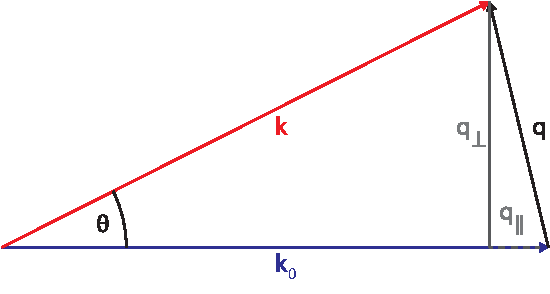
\includegraphics[width=0.5\textwidth]{images/msft.eps}
		\caption[Abbildungstext im Abbildungsverzeichnis]{Abbildungsunterschrift. Abbildung nach \cite{B-SViel}.}
		\label{Abb:BspAbbildung}
	\end{figure} 

	Formel XXX beschreibt einen Algorithmus um das Streubild eines dreidimensionalen Objektes im Fernfeld in der 1. Bornschen Näherung zu berechnen. Diese Methode wird als Multislice Fourier Transformation (MSFT) bezeichnet \cite{barke2015}. Bei dieser wird Mehrfachstreuung ignoriert. Durch nachträgliches Einführen eines zusätzlichen Faktors XXX der die Absorption und Phasenänderung der Welle beim Durchlaufen des Objektes beschreibt, lässt eine grobe Näherung für Absorptionseffekte einzuführen. Eine Implementation des MSFT-Algorithmus liegt in \texttt{simulation/msft.m} vor 

\section{Multislice Propagation}
	Ein alternatives Verfahren zur Simulation XX ist in der Literatur als Multislice oder Beam Propagation bekannt. Dieses Verfahren basiert auf ...
	Die Szene, deren Streubild zu berechnen ist, wird in einzelne Schichten zerlegt.
	Die Ausbreitung der in Szene einfallende ebene Welle wird genähert durch eine Vakuumpropagation von Schicht zu Schicht sowie eine Wechselwirkung mit der Materie der Schicht in einer einzelnen Ebene.
	
	\begin{figure}
		\centering
		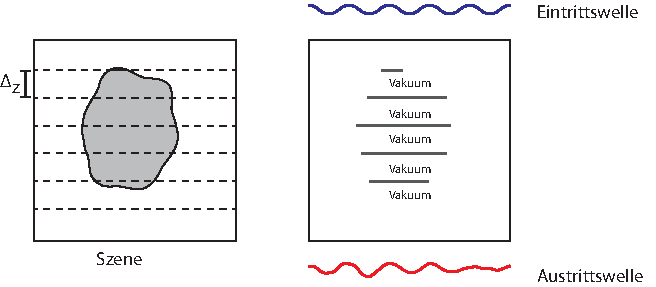
\includegraphics[width=0.75\textwidth]{images/multislice.eps}
		\caption[Abbildungstext im Abbildungsverzeichnis]{Abbildungsunterschrift. Abbildung nach \cite{B-SViel}.}
		\label{Abb:BspAbbildung}
	\end{figure} 
	
	Die Näherung der Vakuumausbreitung durch einen Fresnel-Propagator bringt gegenüber der korrekten Berechnung über die Angular Spectrum Propagation keine numerischen Vorteile. Aus diesem Grund wird im Weiteren im Gegensatz zu \cite{hare}XXX auf diese Näherung verzichtet. Der Algorithmus zur Berechnung der Austrittswelle lautet somit
	\begin{equation}
		Inhalt...
	\end{equation}
	Ist die Austrittswelle bekannt, so ist die weitere ausbreitung zum Detektor eine Vakuumpropagation, die sich entweder mittels Angular Spectrum Propagation berechnen lässt, oder sich durch eine einfache Fouriertransformation in Fraunhofer-Näherung bestimmen lässt. Ersteres Verfahren hat den Nachteil, das es bei einer numerischen Implemantion im Bereich der Szene die gleiche räumliche Rastergröße wie im Bereich des Detektors erfordert, während bei Anwendung der Fernfeld Näherung xxx
\section{Thibaults Multislice}
Thibault stellt in XX einen eigene Formulierung der Multislice-Simulation auf. Ausgehend von der Wellengleichung XX
lässt sich für die Austrittswelle XXX aufstellen.
\begin{equation}
\tilde{\Phi}(z)=\tilde{G}\ast_z\left[\tilde{\delta\eta}\ast_{q_\perp} \tilde{\Phi}\right]
\end{equation}
\begin{equation}
\tilde{G}=\frac{1}{2\pi}\frac{ik^2}{\sqrt{k^2-q_\perp^2}}e^{iz(\kappa-k)}
\end{equation}
unter der Vernachlässigung von Rückstreuung lässt sich das Faltungsintegral als in zwei Integrationsbereiche aufspalten
\begin{equation}
\tilde{\Phi}(z+\Delta z)=
\int_{\Delta z}^{\infty} \tilde{G}(z')\left[\tilde{\delta\eta}\ast_{q_\perp} \tilde{\Phi}\right](z+\Delta z-z')\dif z'
+
\int_{0}^{\Delta z} \tilde{G}(z')\left[\tilde{\delta\eta}\ast_{q_\perp} \tilde{\Phi}\right](z+\Delta z-z')\dif z'
\end{equation}
Für den ersten Summanden gilt

\begin{align*}
&\stackrel{\hphantom{z'\rightarrow z''+\Delta z}}{\hphantom{=}} 
\int_{\Delta z}^{\infty} \tilde{G}(z')\left[\tilde{\delta\eta}\ast_{q_\perp} \tilde{\Phi}\right](z+\Delta z-z')\dif z'\\
&\stackrel{z'\rightarrow z''+\Delta z}{=}
\int_{0}^{\infty} \tilde{G}(z''+\Delta z)\left[\tilde{\delta\eta}\ast_{q_\perp} \tilde{\Phi}\right](z-z'')\dif z''\\
&\stackrel{\hphantom{z'\rightarrow z''+\Delta z}}{=}
e^{i\Delta z(\kappa-k)}\int_{0}^{\infty} \frac{1}{2\pi}\frac{ik^2}{\sqrt{k^2-q^2_\perp}}e^{iz''(\kappa-k)}\left[\tilde{\delta\eta}\ast_{q_\perp} \tilde{\Phi}\right](z-z'')\dif z''\\
&\stackrel{\hphantom{z'\rightarrow z''+\Delta z}}{=}
e^{i\Delta z(\kappa-k)}\tilde{\Phi}(z) \numberthis
\end{align*}
Im zweiten Summanden kann für hinreichend kleine $\Delta z$ das Integral gut durch eine Rieman-Obersumme mit einem einzigen Stützpunkt approximiert werden:
\begin{equation}
\int_{0}^{\Delta z} \tilde{G}(z')\left[\tilde{\delta\eta}\ast_{q_\perp} \tilde{\Phi}\right](z+\Delta z-z')\dif z'
\approx
\Delta z \tilde{G}(\Delta z)\left[\tilde{\delta\eta}\ast_{q_\perp} \tilde{\Phi}\right](z)
\end{equation}
Für den Fehler 
\begin{equation}
\text{Rieman Abschätzung}
\end{equation}
Somit lässt sich in Näherung für die Welle bei $z+\Delta z$
\begin{equation}
\tilde{\Phi}(z+\Delta z)
\approx
e^{i\Delta z(\kappa-k)}
\left[
\tilde{\Phi}(z)+\frac{\Delta z}{2\pi}\frac{ik^2}{\sqrt{k^2-q^2_\perp}}
\right]
\end{equation}
Die numerische Simulation dieser Methode ist in \texttt{simulation/thibault.m} implementiert.


\section{Ergebnisse und Diskussion}
\subsection{Verifizierung}
Zur Verifizierung der vorgestellten Simulationsalgorithmen und deren numerische Implementierungen eignet sich der Vergleich der berechneten Streubilder hinter Kugeln mit den Ergebnissen aus der Berechnung mittels Mie-Streuung. Der vergleich wird für verschiedene Brechzahlen, Kugelradien und Berechnungsauflösungen bei einer Wellenlänge von 1\si{nm} durchgeführt.
Zur Quantifizierung des Vergleichs wird die Summe der Betragsquadrat der Abweichung zwischen den Simulationsdatenpunkten und der Berechnung mittels Mie verwendet.
\subsection{Austrittswellen}
darstellung von interessanten austrittswellen von mehreren objekten und vgl. mit summe aus einzel austrittswellen